We present the integration of Jupyter Notebooks into the MathHub system.

\subsection{Overview}

Our system consists of four components:
\begin{compactitem}
\item A GitLab repository hosting server \url{https://gl.mathhub.info} that provides persistent storage of documents in any format, including their OMDoc representation.
\item A Jupyter Notebook server \url{https://jupyter.mathhub.info} provides web-based IDE for editing interactive documents
\item An MMT instance which uses the OMDoc representations to provides the shared knowledge space and provides a high-level API for it\footnote{
    Technically, each kernel has a separate MMT instance in addition to the primary one. 
    Except for the ephemeral document representing each Notebook, these are identical to the main instance. 
    These exist only to isolate different users from one another, and prevent scenarios where they could unintentionally break each others notebook sessions.  
  }.
\item The MathHub frontend \url{https://mathhub.info} that serves as the main entry point and delegates some subtasks to the former.
  We have extended MathHub front-end with a new new document type presenter for notebooks that gives access to the source, context, statistics, and metadata of notebooks, and provides a ``preview'' and ``interact inline'' views.  
\end{compactitem}

The Jupyter server is an out of the box installation of Jupyter except for additionally supporting our new MMT kernel and a small plugin enabling smoother opening of notebooks via a url. 
Consequently, the integration between the Jupyter and the MathHub frontends is shallow: MathHub opens Jupyter Notebooks in separate tabs or iframes using URLs served by Jupyter.
A deeper integration -- e.g., using Jupyter simply as a JavaScript library in MathHub -- would have been preferable, but is infeasible because Jupyter is primarily designed as a monolithic system.
Recent versions of Jupyter are working Jupyter-as-a-module, so we leave deep integration to future work.

% \begin{oldpart}[
%   TW@all: None of the stuff in this section is implemented as described, and it was no-where on my list to do this short-term. 
%   I will not be able to do so before the paper deadline (or anywhere close to it). 
%   I wasn't really sure what to do here, so for the moment I have commented out the section; I have to look at it again tomorrow
% ]
% \subsection{Notebooks as Standalone Documents}

% The MathHub frontend already provides special interaction functionality for individual document types.
% We used this by making Jupyter Notebooks a new document type; see Figure~\ref{fig:mathhub-NB} for an example.
% When displaying a known document type, the frontend shows multiple tabs.
% For Notebooks, these are the following:
% \begin{compactenum}[\em i\rm)]
% \item \textsf{view} gives a preview of the notebook, essentially the computation cells without output, pre-rendered for static serving without involving Jupyter at all. 
% \item \textsf{run/edit} opens the respective notebook on the Jupyter server for execution and editing.
% Any changes to the Notebook made from within Jupyter can be committed back to the Git repository. 
% \item \textsf{metadata} (this is the tab open in Figure~\ref{fig:mathhub-NB}), shows the metadata provided by the Jupyter kernel and the repository. 
% \item \textsf{source} provides access to the document source; here simply a link to the notebook file in the Git repository.
% \item \textsf{statistics} shows statistical information about the notebook, its corresponding MMT document, and its connections with other MMT documents in the background knowledge base.
% \item \textsf{graph} links to graph-based visualizations of the document including the theory graph, declaration graph, and dependency graph, using our TGView system, a canvas-based in-browser visualizer for knowledge graph information~\cite{RupKohMue:fitgv17}.
% \end{compactenum}
% This integration combines the interactive features of the Jupyter server with the knowledge management facilities on MathHub. In the future, we plan to integrate the notebook diff/patch \textsf{nbdime} developed in OpenDreamKit to extend the knowledge management facilities. 

% \begin{figure}[ht]\centering
%   \fbox{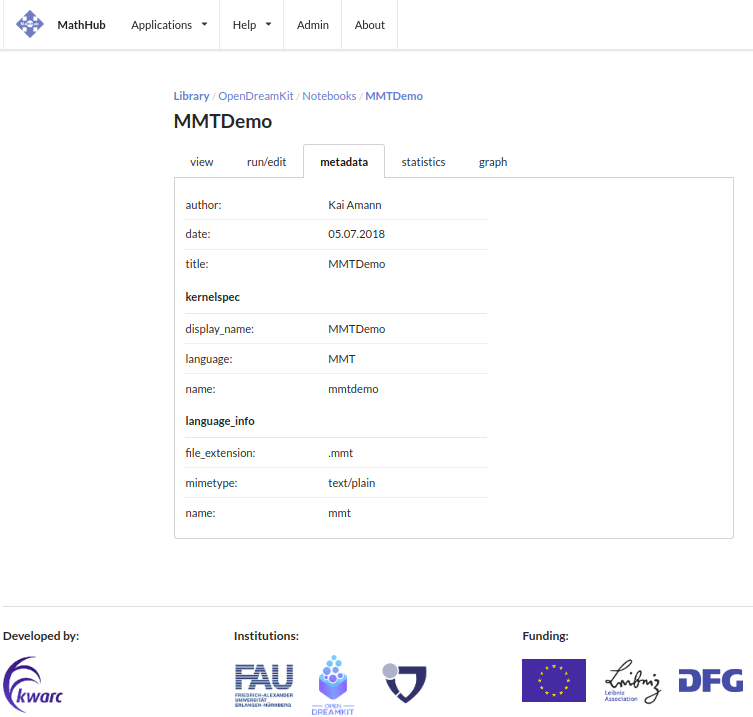
\includegraphics[width=13cm]{../D4.11/NB-Mathhub}}
%   \caption{A Jupyter Notebook in MathHub (Metadata)}\label{fig:mathhub-NB}
% \end{figure}

% \end{oldpart}

\subsection{Notebooks as Parts of Static Documents}

To interact dynamically with content in arbitrary MathHub documents, we added a new feature that creates a new ephemeral Jupyter Notebook and allows accessing it from the current document.
Importantly, the new Notebook is pre-filled with an import of the current context so that users can Here we can feed the document context information into the interior notebook.

\begin{figure}[ht]\centering
  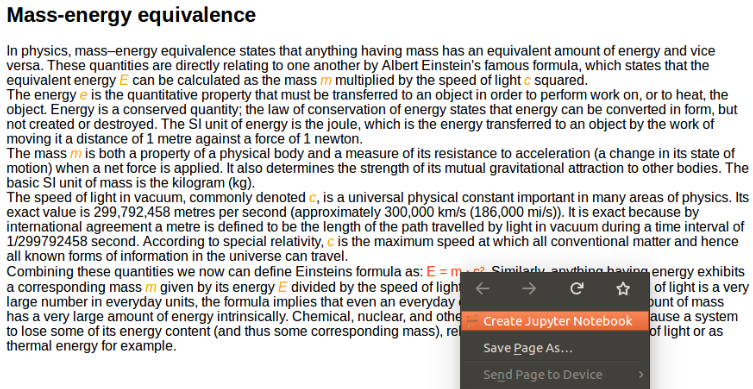
\includegraphics[width=15cm]{../D4.11/conversionHTML}
  \caption{HTML document and the context menu for converting}\label{fig:conversionHTML}
\end{figure}

Figure~\ref{fig:conversionHTML} shows a scientific HTML document that contains the equation $E=mc^2$.
The user can use the context menu to trigger the notebook generation on this formula.
The context menu is generated using JavaScript that picks up on annotations of formulas with specific CSS classes.
Currently the author has to manually annotate the formulas, but we are working on a mechanism to automatically create it from the document context.
The data is then sent to our Jupyter installation using appropriate URL parameters. 

Figure~\ref{fig:conversionNotebook}\ednote{Update this screenshot} shows the notebook created by our tool.
Note that the generated notebook starts with several \texttt{include} declarations that import the context of the formula.
These are generated by MathHub to obtain a minimal standalone MMT theory in which the respective formula is well-formed. 
It then continues by making use of the active computation widget we presented above. 

If desired, the notebooks can be easily uploaded to the Jupyter server, stored persistently in the repository server, or evaluated in a locally deployed version of the system per drag-and-drop.

\begin{figure}[ht]\centering
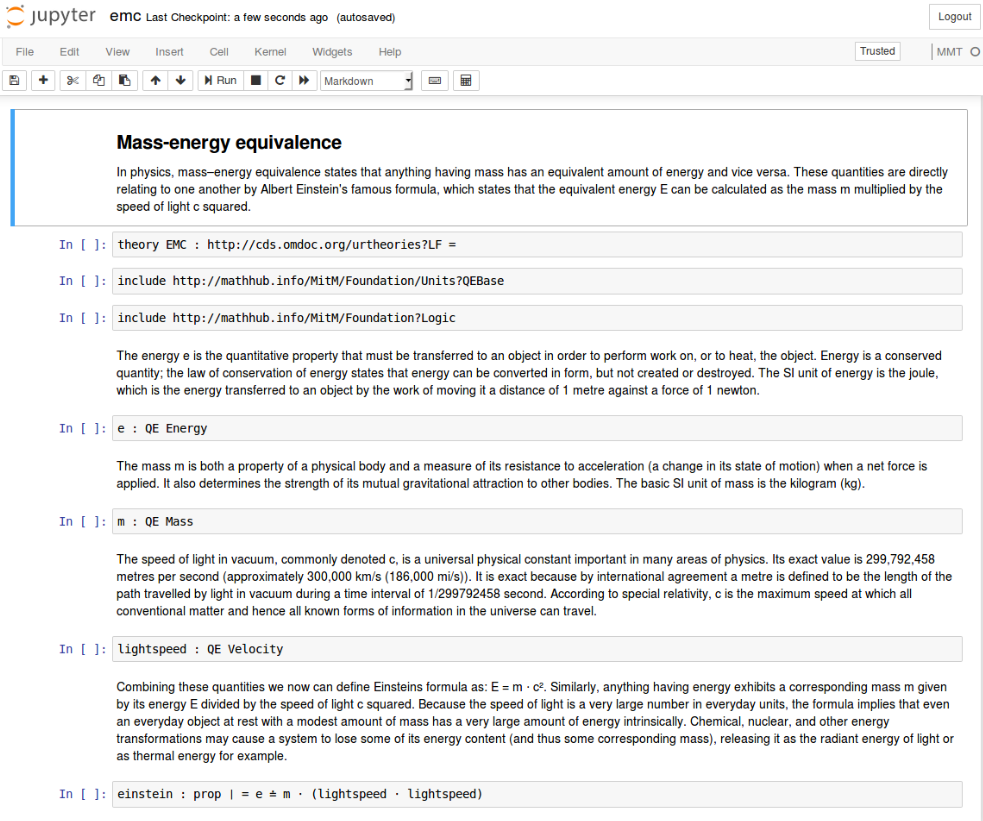
\includegraphics[width=15cm]{../D4.11/conversionNotebook}
\caption{The resulting Jupyter notebook}
\label{fig:conversionNotebook}
\end{figure}

%%% Local Variables:
%%% mode: latex
%%% mode: visual-line
%%% fill-column: 5000
%%% TeX-master: "paper"
%%% End:

%  LocalWords:  Jupyter ednote compactenum textsf texttt visualizations RupKohMue:fitgv17 nbdime centering fbox includegraphics NB-Mathhub compactitem oldpart
